\documentclass{article}%You can define the type of paper here.
%%Useful packages that I commonly use.
\usepackage[numbers]{natbib}%Bibliography package (help at http://merkel.zoneo.net/Latex/natbib.php).
\usepackage{url}%Package to highlight url.
\usepackage{times}%Sets font to be times.
\usepackage{siunitx}
\usepackage{alltt}%Allows the use of verbatim (good for printing out code).
\usepackage{graphicx}%Used to import images.
\usepackage{amsmath, amssymb, amscd}%Contains the AMS expanded math symbols library.
\usepackage{algorithm, algorithmic} %pseudo-code
%%For those who want smaller margins, you can use this:
\usepackage[top=1in, bottom=1in, left=1in, right=1in]{geometry}


\begin{document}

%% Title =======================================================================

\title{Firn Densification Model}
\author{Cummings, Evan \and Davis, Tyler \and Brinkerhoff, Douglas}
\maketitle
\begin{center}

\includegraphics[width=4.455666122085252in]{images/logoPlain.png}
\end{center}

\twocolumn


%% Introduction ================================================================
\section{Introduction}

The top layer of snow on a glacier or ice sheet increases in density as depth increases.  Several models have been created to simulate this process, some based on temperature and others based on enthalpy.  I have re-created these models with the finite-element software package FEniCS.

%% Temperature =================================================================
\section{Temperature Solution}

We begin with the standard heat-transport equation (Patterson, 2001

  $$
  \rho c_i \frac{\partial T}{\partial t} = 
    k_i \frac{\partial^2 T}{\partial z^2} +
    \left( \frac{dk_i}{dt} - \rho c_i w \right) \frac{\partial T}{\partial z}
  $$
with heat sources from the deformation of ice ommitted, $\rho$ density, $c_i$ heat capacity, $k_i$ thermal conductivity, $w$ vertical velocity, and $T$ temperature of firn.  To solve the total derivative $dk_i/dt$ we must apply the chain rule
  $$
  \frac{dk_i}{dz} = 
  \frac{\partial k_i}{\partial \rho} \frac{\partial \rho}{\partial z} + 
  \frac{\partial k_i}{\partial T} \frac{\partial T}{\partial z}.
  $$
The thermal conductiviy of ice is defined by Arthern et. al, 1998 as
  $$k_i = 2.1 \left(\frac{\rho}{\rho_i}\right)^2,$$
and gives
  $$
  \frac{\partial k_i}{\partial \rho} = 
    4.2 \frac{\rho}{\rho_i^2}
  $$
and
  $$
  \frac{\partial k_i}{\partial T} = 
    \frac{4.2}{\rho_i^2} \left( \frac{\partial \rho}{\partial T} \right).
  $$
Patterson, 2001 defined $\rho$ in terms of $T$ and from this can be derived
  $$
  \frac{\partial \rho}{\partial T} = 
    \SI{5.6e-2} \exp ((\SI{-5.7e-3})T).
  $$
The vertical velocity of ice, $w$, is directly proportional to the accumulation, $b$,
  $$
  w = -\frac{b}{\rho}
  $$
with $b$ in units of kg m$^{-2}$ s$^{-1}$.  The densification process is defined with the material derivative
  $$\frac{d \rho}{dt} = \frac{\partial \rho}{\partial t} + 
    w\frac{\partial \rho}{\partial z}.$$
Arthern et. al, 2010 described this total derivative with the formula  
  $$
  \frac{d \rho}{dt} = 
  \begin{cases}
   c_0(\rho_i - \rho), &\rho <= 550\ kg\ m^{-3}\\
   c_1(\rho_i - \rho), &\rho > 550\ kg\ m^{-3}
  \end{cases}.$$
Zwally and Li, 2002 defined the multiplying constant $c$ with an arrhenius-type relation
  $$
  c_0 = c_1 = 
  b \beta(T)\left(\frac{\rho_i}{\rho_w}\right)
  K_{0G}(T)\exp \left( -\frac{E(T)}{RT} \right),
  $$
with $K_{0G}(T) \exp(-E(T)/(RT)) = 8.36T^{-2.061}$, and $\beta(T)$ a smoothing function to match a desired density rate.  Arthern et. al 2010 developed a semi-empirical formula by coupling the rate equations for Nabarro-Herring creep and normal grain-growth : 
  $$
  \begin{cases}
    c_0 = M_0 bg\frac{k_{c0}}{k_g}\exp\left(-\frac{E_c}{RT} + 
          \frac{E_g}{RT_{avg}}\right)\\
    c_1 = M_1 bg\frac{k_{c1}}{k_g}\exp\left(-\frac{E_c}{RT} + 
          \frac{E_g}{RT_{avg}}\right)
  \end{cases},
  $$
with the creep coefficients defined as
  $$
  \begin{cases}
    k_{c0} = \SI{9.2e-9} m^3\ s\ kg^{-1} \\
    k_{c1} = \SI{3.7e-9} m^3\ s\ kg^{-1}  
  \end{cases}
  $$
and $M$ defined by Ligtenberg et. al 2011 to better fit with observed densification rates in higher-temperature environments :
  $$
  \begin{cases}
    M_0 = 2.366 - 0.293\ln(b*\SI{1e3})\\
    M_1 = 1.435 - 0.151\ln(b*\SI{1e3})
  \end{cases}.
  $$
Within the same paper a firn surface density expression from data was given :
  $$ \rho_s = -151.94 + 1.4266(73.6 + 1.06T_s + 0.0669A + 4.77V_a).$$


%% Enthalpy ====================================================================
\section{Enthalpy Solution}

As stated in Aschwanden et. al 2012, we take 'enthalpy' to be synonymous with 'internal energy' due to the exclusion of work done with changing volume.  The equation used here is the shallow-enthalpy :
	$$
  \rho \frac{\partial H}{\partial t} = \frac{\partial}{\partial z} 
    \left( 
      \begin{Bmatrix}
        K_i(H), &\text{Temperate}\\
        K_0, &\text{Cold}
      \end{Bmatrix}
      \frac{\partial H}{\partial z} 
    \right) + w \rho \frac{\partial H}{\partial z}.
  $$
Strain heating has been neglected and the advective term $w \rho\ \partial H / \partial z$ has been added.  The coefficient for temperate ice is 
  $$K_i(H) = \frac{k_i}{c_i}.$$
The coefficient for cold ice is
  $$K_0 = \frac{1}{10}K_i(H).$$
Temperate firn is defined as firn with $H > H_s$ and cold firn $H <= H_s$, with
  $$H_s = \int_{T_0}^{T_m}{c_i(T)}dT$$ 
where $T_m = 273.15$ K and $T_0 = 0.0$ K.  The enthalpy can be found with a constant heat capacity of $2009$ J kg$^{-1}$ K$^{-1}$ with the linear equation
  $$
  H = 
  \begin{cases}
    c_i(T - T_0), &\text{where } T <= T_m\\
    c_i(T_w - T_0) + \omega L_f,  &\text{where } T > T_m
  \end{cases}
  $$
where $L_f$ is the latent heat of fusion and $\omega$ represents the water content percentage of firn given by
  $$\omega L_f = H - c_i(T_w - T_0).$$
It is conveinent to find the temperature :
  $$T = \frac{H}{c_i}.$$
The density equations remain the same as the temperature solution, and the surface density at time index $n+1$ can be described as : 
  $$\rho_s^{n+1} = \rho_b^{n+1} d_p + \rho_s^{n} (1 - d_p),$$
where
  $$\rho_b^{n+1} = \rho_b^{n-1} + \Delta \omega_s \rho_b^n,$$
  $$\Delta \omega_s = \omega_s^{n} - \omega_s^{n-1},$$ 
  $$d_p = \frac{d_n}{l_s},$$
  $$d_n = w_sdt,$$
$l_s$ is the length of the surface node, and
  $$
  \rho_b^n = 
  \begin{cases}
    \rho_w - \rho_i\ \text{kg m}^{-3},  &T <= T_w\\
    \rho_w\ \text{kg m}^{-3}, &T > T_w
  \end{cases}.
  $$
\begin{figure}[H]
	\centering
		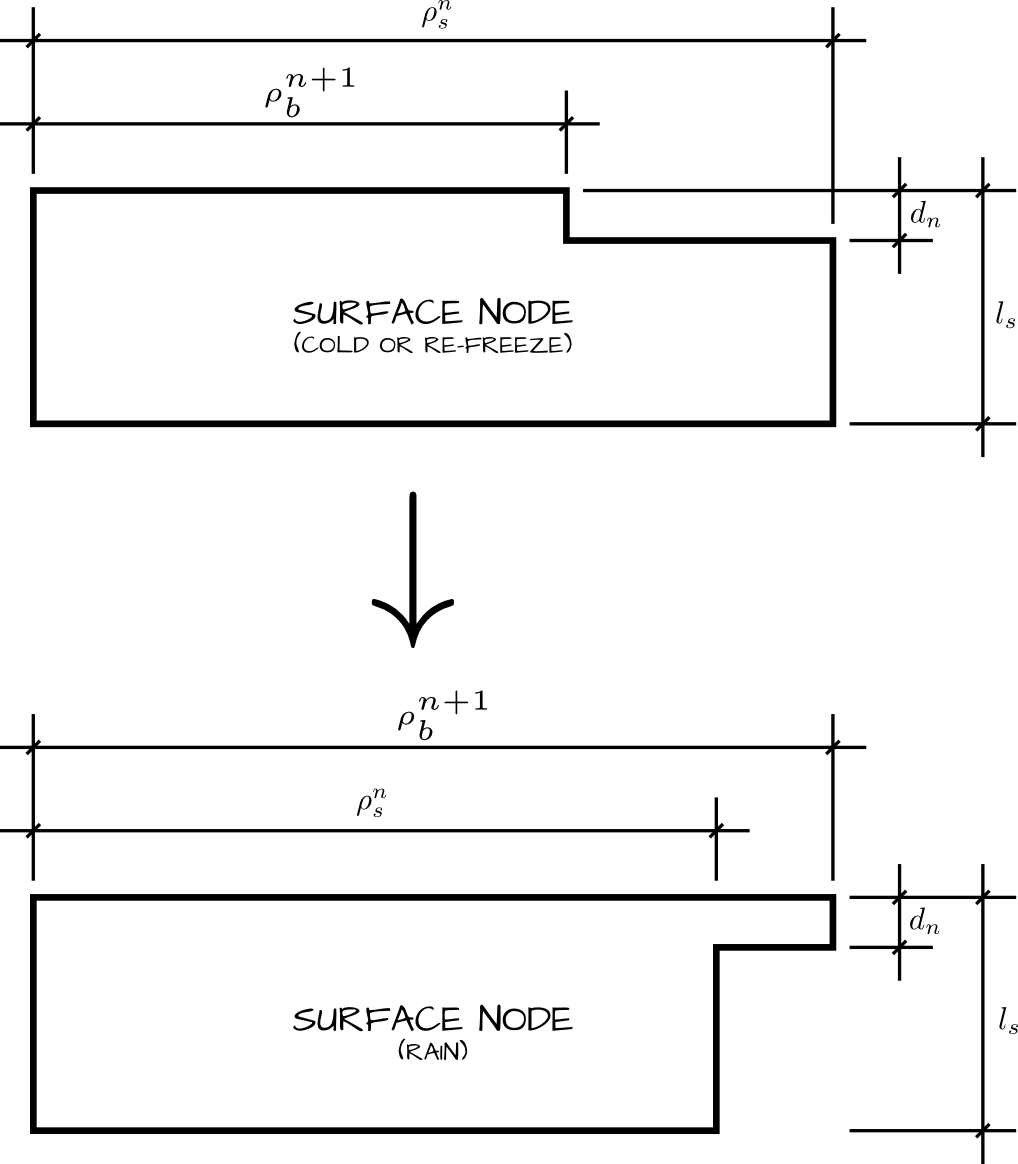
\includegraphics[width=0.42\textwidth]{images/surfaceDensity.png}
	\label{fig:500 year orbit}
	\caption{Evolution of surface node density}
\end{figure}

%% Method ======================================================================
\section{Finite Element Method}

This section will focus on the enthalpy solution; solving these equations with FENicS is done with Galerkin's method which requires finding the weak formulation :
  $$
    0 =
    \int_{\Omega} 
      \begin{Bmatrix}
        K_i(H)\\
        K_0
      \end{Bmatrix}
      \nabla^2 H \psi\ d \Omega 
    + \int_{\Omega}w \rho \nabla H \psi\ d \Omega
  $$
  $$
    - \int_{\Omega} {\rho \frac{\partial H}{\partial t}} \psi\ d \Omega.
  $$
Here we have integrated over the entire domain, $\Omega$, and multiplied by a test function $\psi$.  After integrating the diffusive term by parts this becomes
  $$
    f_H =
    - \int_{\Omega} 
        \begin{Bmatrix}
          K_i(H)\\
          K_0
        \end{Bmatrix}
        \nabla H \nabla \psi\ d \Omega 
    + \int_{\Omega}w \rho \nabla H \psi\ d \Omega
  $$
  $$
    - \int_{\Omega} {\rho \frac{\partial H}{\partial t}} \psi\ d \Omega.
  $$
We can descritize the enthalpy time-differential with the second-order accurate backward-difference formula
  $$\frac{\partial H}{\partial t} = \frac{H^{k-2} - 4H^{k-1} + 3H}{2dt},$$
with superscripts referring to time index.  This equation can be represented in FENicS as :
\small
\begin{alltt}
f_H = (rho*(H_2 - 4*H_1 + 3*H)/(2*dt)*psi 
      + k/c*Kcoef*inner(grad(H), grad(psi))
      + rho*w*grad(H)*psi)*dx
\end{alltt}
\normalsize
The variable \texttt{Kcoef} is a coefficient vector which will be updated dynamically depending on the temperature of firn (either $1.0$ or $0.1$).

The weak form for density is found similarly :
  $$
  f_{\rho} = 
    \int_{\Omega} \frac{\partial \rho}{\partial t}\phi\ d \Omega + 
    \int_{\Omega} w\nabla \rho \phi\ d \Omega -
    \int_{\Omega}\frac{d \rho}{dt}\phi\ d \Omega.
  $$
With the partial-time-differential of density defined indentically to the enthalpy equation, this can be represented in FENicS with the Arthern et. all 2010 densification equation as :
\small
\begin{alltt}
c      = b*g*rhoCoef/kg * 
         exp(-Ec/(R*T) + Eg/(R*Tavg))
drhodt = c*(rhoi - rho)
f_rho  = ((rho_2 - 4*rho_1 + 3*rho)/(2*dt) 
         - drhodt + w*grad(rho))*phi*dx 
\end{alltt}
\normalsize
The variable \texttt{rhoCoef} is another dynamically-updated-coefficient vector and is either $k_{c0}$ or $k_{c1}$ depending upon the density at the node.

We can define the function space for the entire non-linear problem as 
  $$
    U = \Omega \times \Omega,
  $$
with corresponding trial and test functions respectively defined as
  $$
    v, u \subset U.
  $$
The test functions for each function can now be described as
  $$
    \psi, \phi \subset u.
  $$
In FENicS these spaces can be defined by this :
\small
\begin{alltt}
V         = FunctionSpace(mesh, 
                          'Lagrange', 
                          1)
MV        = V*V
h         = Function(MV)
H,rho     = split(h)    
dh        = TrialFunction(MV)
dH, drho  = split(dh)
j         = TestFunction(MV)
psi, phi  = split(j)
\end{alltt}
\normalsize

We define the entire function as 
  $$
    f = f_H + f_{\rho}.
  $$
Solving this system can be accomplished with \emph{Newton's Method} which requires derivation of the Jacobian :
  $$
    J = \frac{\partial f}{\partial v}.
  $$
In FENicS this becomes :
\small
\begin{alltt}
f  = f_H + f_rho
J  = derivative(f, h, dh)
\end{alltt}
\normalsize


%% Boundary Conditions =========================================================
\section{Boundary Conditions}

The cyclical enthalpy boundary condition for the surface can be simulated with 
  $$
    H_s = c_i ( T_s - T_0 ),
  $$
  $$
    T_s = T_{avg} + \alpha \sin(\omega t),
  $$
where $\alpha$ is the amplitude of temperature variation and $\omega = 2\pi / spy$ is the frequency.  The surface-density boundary condtion can be likewise described as (see figure 1) : 
  $$
    \rho_s^{n+1} = \rho_b^{n+1} d_p + \rho_s^{n} (1 - d_p).
  $$
Both of these can be created with FENicS with
\small
\begin{alltt}
code = 'c*(Tavg + 9.9*sin(omega*t) - T0)'
Hs   = Expression(code, c=cp, Tavg=Tavg, 
                  omega=freq, t=t0, T0=T0)

code = 'dp*rhon + (1 - dp)*rhoi'
rhoS = Expression(code, rhon=rhosi, 
                  rhoi=rhosi, dp=1.0)

def surface(x, on_boundary):
  return on_boundary and x[0] == zs

Hbc  = DirichletBC(MV.sub(0), Hs, surface)
Dbc  = DirichletBC(MV.sub(1), rhoS, surface)
\end{alltt}
\normalsize
Within the time-loop the variables \texttt{t}, \texttt{rhon}, \texttt{rhoi}, and \texttt{dp} can be updated as needed.

Now all that is left is to iterate through time and call the \texttt{solve} method at each step :
\small
\begin{alltt}
solve(f == 0, h, [Hbc, Dbc], J=J)
\end{alltt}
\normalsize
The use of the \texttt{solve} function in this way chooses \emph{Newton's Method} by default and minimizes the residual of \texttt{f}.  The boundary conditions are updated by specifing the list \texttt{[Hbc, Dbc]}.


%% Model Parameters ============================================================
\section{Model Parameters}

Within the time-loop there are a number of parameters which need to be updated.  Taking into account conservation of mass, the height $l$ of each node must be re-calculated :
  $$l^{n+1} = l^n \frac{\rho_{ini}}{\rho},$$
where $\rho_{ini}$ is the density of the firn column when the system was initialized.  With the height of the nodes calculated, the z-positions may be found by iterating through the heights and setting the z vector's correspoding cell equal to the current sum.  After sucessfull calculation the FENicS \texttt{mesh} object must have its coordinates refreshed.  These tasks may be completed with the following code :
\small
\begin{alltt}
lnew     = l*rhoin[index] / firn.rho[index]
zSum     = zb
zTemp    = zeros(n)
for i in range(n)[1:]:
  zTemp[i] = zSum + lnew[i]
  zSum    += lnew[i]
firn.z[index] = zTemp
mesh.coordinates()[:,0] = firn.z
\end{alltt}
\normalsize
The variable \texttt{index} is an array of positions corresponding to the correct ordering of the nodes, necessarry after mesh refinement; \texttt{zb} is the z-position of the base of the firn column which does not change and \texttt{n} is the nuber of nodes.

The height $s$ at time index $n$ of the original surface may be calculated as follows :
  $$s^{n} = (z_s - z_b) \frac{s^{n-1} - z_b}{z_{s} - z_b} + w_s dt.$$
This maintains the relative location of the original surface to the current surface and moves downward proportional to $w$.

For all operations it is conveinent to store all the state data from the simulation in a class object for ease of access.  For this purpose the \texttt{firn} class was created and contains the signature 
\small
\begin{alltt}
firn(self, H, T, rho, omega, w, 
     k, c, z, index)
\end{alltt}
\normalsize
with \texttt{z} the node z-positions as defined above, \texttt{index} index of re-ordered mesh locations, and other variables as described earlier in the paper.


%% Variable Definition =========================================================
\section{Variable Definitions}

Many variable are used in this simulation and many do not change.  These are defined below :\\

\noindent\textbf{Constants :}

\footnotesize
\noindent\begin{tabular}{lccc}
\hline
Var. & Value & Units & Description\\
\hline
$g$ & $9.81$ & m s$^{-2}$ & gravitational acceleration\\
$R$ & $8.3144621$ & J mol$^{-1}$ K$^{-1}$ & gas constant\\
$spy$  & $31556926$ & s & seconds per year\\
$\rho_i$ & $917$ & kg m$^{-3}$ & density of ice\\
$\rho_w$ & $1000$ & kg m$^{-3}$ & density of water\\
$\rho_m$ & $550$ & kg m$^{-3}$ & critical density value\\
$k_i$  & $2.1$ & W m$^{-1}$K$^{-1}$ & thermal conductivity of ice\\
$c_i$  & $2009$ & J kg$^{-1}$K$^{-1}$ & heat capacity of ice\\
$T_w$  & $273.15$ & K & triple point of water\\
$k_g$ & \SI{1.3e-7} & m$^2$s$^{-1}$ & grain growth coefficient\\
$E_c$ & \SI{60e3} & J mol$^{-1}$ & act. energy for water in ice\\
$E_g$ & \SI{42.4e3} & J mol$^{-1}$ & act. energy for grain growth\\
\hline
\end{tabular}
\normalsize\\

\noindent\textbf{Model :}

\footnotesize
\noindent\begin{tabular}{lcc}
\hline
Var. & Units & Description\\
\hline
$\rho_{si}$ & kg m$^{-3}$ & initial density at surface\\
$b$  & kg m$^{-2}$s$^{-1}$ & surface accumulation\\
$A$  & mm a$^{-1}$ & surface accumulation\\
$V_a$  & m s$^{-1}$ & mean annual wind speed\\
$T_{avg}$ & K & average annual temperature\\
$T_{s}$ & K & firn surface temperature\\
$z_s$ & m & surface start z-location\\
$z_b$ & m & firn base z-location\\
$z_{s0}$ & m & previous time-step's surface\\
$dz$ & m & initial z-spacing\\
$l$ & m & vector of node heights\\
$dt$ & s & time-step\\
$t_0$ & s & begin time\\
$t_f$ & s & end-time\\
\hline
\end{tabular}
\normalsize\\

\noindent\textbf{Enthalpy-specific :}

\footnotesize
\noindent\begin{tabular}{lccc}
\hline
Var. & Value & Units & Description\\
\hline
$T_0$ & $0.0$ & K & reference temperature\\
$L_f$ & \SI{3.34e5} & J kg$^{-1}$ & latent heat of fusion\\
$H_s$ & $c_i(T_w - T_0)$ & J kg$^{-1}$ &  Enthalpy of ice at $T_w$\\
\hline
\end{tabular}
\normalsize\\


%% Verification ================================================================
\section{Verification of Program}


%% Interpretation ==============================================================
\section{Interpretation}


\end{document}
%%Compile with pdflatex file.tex



